\subsection{Purpose and Procedure}


The objective of this experiment was to measure the wavelength of a red laser beam (\(\lambda\)) using a Michelson interferometer. The laser wavelength was determined by analyzing interference fringes produced by the recombination of two coherent light beams on a screen.  

\begin{figure}[h]
    \centering
    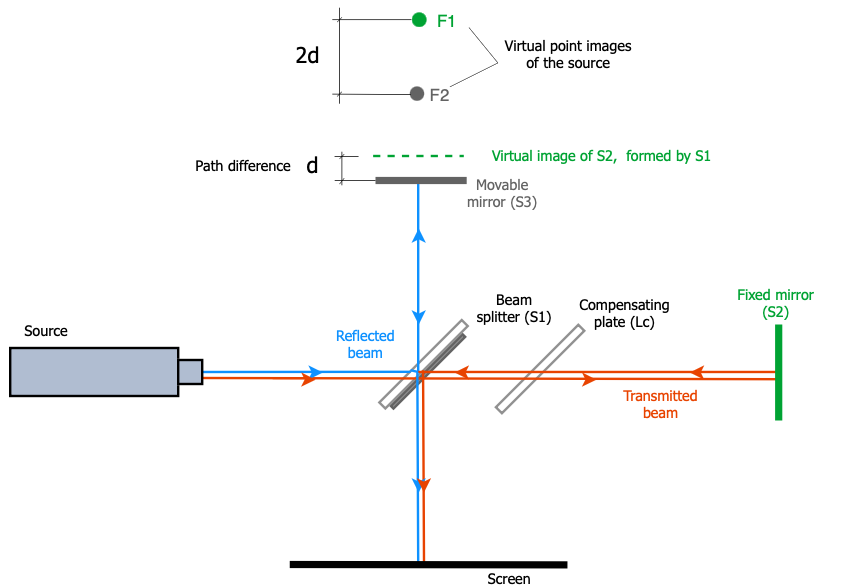
\includegraphics[width=0.9\linewidth]{The_Michelson_interferometer/finalimageupd3.png}
    \caption{A schematic diagram of the Michelson interferometer}
    \label{fig:michelson}
\end{figure}

The Michelson interferometer consisted of the following key components: Beam Splitter (S1) divides the incident laser beam into two orthogonal paths. Fixed Mirror (S2) reflects one of the split beams. Movable Mirror (S3) adjusted using a micrometer screw to vary the optical path difference. Compensating Plate (Lc) ensures equal optical path lengths for the two beams.  

The beam reflected by S2 traverses S1 once, while the beam reflected by S3 traverses S1 three times. The system creates two virtual coherent point sources (F1 and F2), which produce interference fringes on the screen when their light paths recombine.  

Before any interference data were recorded, it was critical to ensure that mirrors \(S_2\) and \(S_3\) were oriented at a right angle. To achieve this, a laser beam was directed onto the beam splitter so that it reflected off both \(S_2\) and \(S_3\). The superimposed beams on the screen were brought into coincidence by adjusting the screws on \(S_2\). A converging lens was then placed in the beam’s path; if the mirrors were orthogonal, circular (rather than elliptical) fringes were observed. Minor tilt corrections were applied until all elliptical distortions disappeared, confirming a \(90^\circ\) alignment. 

%The micrometer screw controlling \(S_3\) has a sensitivity of \(2\,\mu\mathrm{m}\).

%the reflected spots are superimposed and the observed fringes become circular, confirming the 90° orientation.
%The micrometer screw controlling S3 has a sensitivity of \(2 \, \mu \text{m}\). 

The displacement of S3 (\(\Delta x\)) was measured as a difference between two micrometer readings, each with an uncertainty of \(2 \, \mu \text{m}\). For the wave calculation, the refractive index \(n_a\) is taken as 1, introducing a negligible error since \(n_a \approx 1.00027\). 
The wavelength was calculated using the formula:  

\[
\lambda = \frac{2 n_a\Delta x}{N} \approx \frac{2 \Delta x}{N}\,
\]  

where \(N\) is the number of fringes observed during the displacement.  

\subsection{Analysis and Error Evaluation}

The measured mirror displacements (\(\Delta x\)), calculated as 1/5 of the micrometer screw readings, the fringe counts (\(N\)), and the calculated wavelengths (\(\lambda\)) are presented in the table below.

\begin{table}[!htbp]
    {\par\centering
    \begin{tabular}{ccccc}
        \hline
        Measure & $\Delta x \text{ (µm)}$ & $N$ & $\lambda$ \text{(nm)} & $ \varepsilon_\lambda\ $ \text{(nm)} \\
        \hline
        1   &   42& 130&   646.2 & 43.8\\
        2   &   42& 130&   646.2 & 43.8\\
        3   &   41& 130&   630.8 & 43.8\\
        4   &   40& 130&   615.4 & 43.8\\
        5   &   48& 150&   640.0 & 38.0\\
        \hline
    \end{tabular}
    \par}
    \caption{Measurement of the Wavelength of Laser Light}
\end{table}


%The total uncertainty in the wavelength (\(\varepsilon_\lambda\)) arises from uncertainties in the measured displacement (\(\varepsilon_{\Delta x}\)) and the fringe count (\(\varepsilon_N\) = 1). Since \(\Delta x\) is measured as a difference of two micrometer readings, each with an uncertainty of \(2 \, \mu \text{m}\), the total uncertainty in \(\Delta x\) is:  
%\[
%\varepsilon_{\Delta x} = \sqrt{(2 \, \mu \text{m})^2 + (2 \, \mu \text{m})^2} = 2.83 \, \mu \text{m}
%\] \[
%\varepsilon_\lambda^2 = \left(\frac{\partial \lambda}{\partial \Delta x} \varepsilon_{\Delta x}\right)^2 + \left(\frac{\partial \lambda}{\partial N} \varepsilon_N\right)^2,
%\] where:  \[
%\frac{\partial \lambda}{\partial \Delta x} = \frac{2}{N}, \quad %\frac{\partial \lambda}{\partial N} = -\frac{2 \Delta x}{N^2}.
%\]

%The standard deviation of the individual measurements is:  
%\[
%\sigma = \sqrt{\frac{\sum (\lambda_i - \bar{\lambda})^2}{n-1}} = 13.0 \, \text{nm}
%\]  
%The standard deviation of the mean is:  
%\[
%\sigma_{\text{mean}} = \frac{\sigma}{\sqrt{n}} = 5.8 \, \text{nm}
%\]  


%While the theoretical uncertainty is small, it only accounts for errors in \(\Delta x\) and \(N\), assuming no systematic or random errors. The standard deviation of the mean provides a more realistic estimate, capturing variability between measurements and reflecting the true precision of the experiment.  




To address the large uncertainty (\(\varepsilon_\lambda\)) compared to the standard deviation of the mean (\(\sigma_{\text{mean}}\)), the weighted averaging method was applied. This approach accounts for the uncertainties of individual measurements, providing a robust final estimate for the wavelength.

The weighted mean wavelength is calculated as:
\[
\bar{\lambda} = \frac{\sum \left(\frac{\lambda_i}{\varepsilon_{\lambda,i}^2}\right)}{\sum \left(\frac{1}{\varepsilon_{\lambda,i}^2}\right)},
\]
with the uncertainty:
\[
\varepsilon_{\bar{\lambda}} = \sqrt{\frac{1}{\sum \left(\frac{1}{\varepsilon_{\lambda,i}^2}\right)}}.
\]

The uncertainty for each measurement, \(\varepsilon_{\lambda,i}\), was calculated using:
\[
\varepsilon_{\lambda,i} = \sqrt{\left(\frac{2}{N} \varepsilon_{\Delta x}\right)^2 + \left(-\frac{2 \Delta x}{N^2} \varepsilon_N\right)^2},
\]
where \(\varepsilon_{\Delta x} = 2.83 \, \mu\mathrm{m}\) and \(\varepsilon_N = 1\).

The final result is:
\[
{\lambda} = (636.0 \pm 19.0) \, \text{nm}
\]

This value is consistent with the nominal wavelength of \(632.8 \, \text{nm}\) within the experimental uncertainty.
